\chapter{Étude et réalisation du Sprint 2}
% \setcounter{tocdepth}{2}
% \startcontents[chapters]
% \printcontents[chapters]{}{1}{\section*{Sommaire}}
\etocsettocstyle{\section*{Sommaire}}{}
\localtableofcontents

\newpage
\section{Introduction}
\noindent
Aprés avoir terminé le Sprint 1 du chapitre 4 qui tratait la recherche des produits dans la langue Française, nous entamons maintenant le Sprint 2 qui va aborder la recherche en Arabe en dialecte Tunisien, et ensuine l'Arabe Traditionnel.

\section{Backlog du Sprint 2}
\begin{table}[H]
	\centering

	\begin{tabularx}{\textwidth}{|c|X|c|c|}
		\hline
		\rowcolor{blue!20}
		\textbf{ID} & \textbf{Scénario}                                                                                     & \textbf{Priorité} & \textbf{Complexité} \\ \hline
		1           & En tant qu'un client, visiteur, je veux saisir ma terme de recherche en Arabe en dialecte Tunisien pour chercher le(s) produit(s) & 1                 & 7                  \\ \hline

	2           & En tant qu'un client, visiteur, je veux saisir ma terme de recherche en Arabe Traditionnel pour chercher le(s) produit(s) & 2                 & 6 \\ \hline
	3           & En tant qu'un client, visiteur, je veux des produits similaires comme des suggestions. & 3                 & 6 \\ \hline
	\end{tabularx}
	\caption{Backlog du Sprint 2}
	\label{tab:sprint2}
\end{table}

\section{Spécification fonctionnelle}
\noindent
Dans cette partie, on va expliquer les différentes fonctionnelités du Sprint 2 à travers le diagramme de cas d'utilisation. Puis en va exposer les différents scénarios de notre cas d'utilisation à travers des descriptions textuelles.

\section{Diagramme de cas d'utilisation général}
\noindent
La figure ~\ref{fig:recherchearabe} illustre le diagramme de cas d'utilisation gènèral de notre premier sprint, qui est la recherche en Français.

\begin{figure}[H]
	\centering
	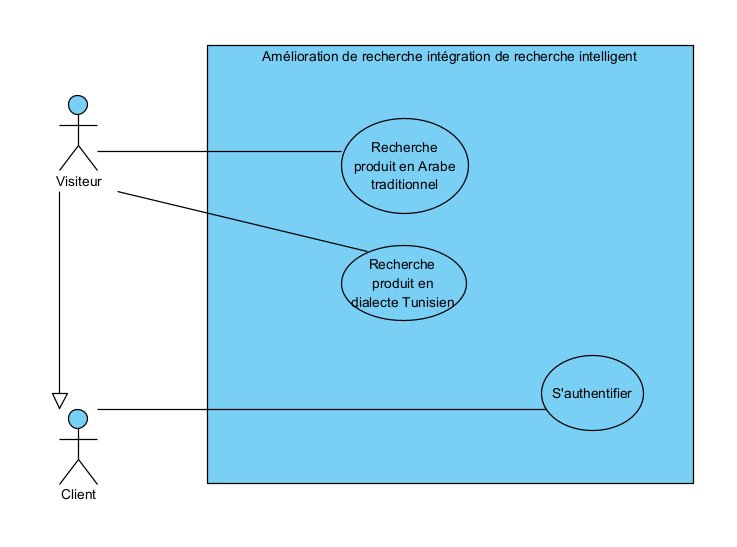
\includegraphics[width=1\textwidth]{logos/cusprint2.png}
	\caption{Diagramme de cas d'utilisation général du Sprint 2}
	\label{fig:recherchearabe}
\end{figure}

\section{Description textuelle des cas d’utilisations}
Une fois les divers cas d'utilisation présentés, nous examinerons de plus près certains
d'entre eux en fournissant la description textuelle de certains d'entre eux.

\newpage
\subsection{Description textuelle du CU « Rechercher produit en Arabe traditionnel »}
\noindent
\textbf{Titre:} Rechercher produit en Arabe traditionnel \\
\textbf{Résumé:} Le client saisit son terme de recherche en Arabe traditionnel, en cliquant sur la boutton pour rechercher le(s) produit(s) qu'il veut chercher. \\
\textbf{Acteur Principal:} Client \\
\textbf{Précondition:} \begin{enumerate}
	\item Le client (ou le visiteur) sont sur la page de recherche
	\item Le client (ou le visiteur) a saisi son terme de recherche en Arabe traditionnel
	\item Le client (ou le visiteur) a cliqué sur "Rechercher"
\end{enumerate}
\textbf{Postcondition:} Le(s) produit(s) que le client cherche est renvoyé, si'il n'existe pas, le systéme renvoie des produits similaires comme suggestion. \\
\textbf{Scénario de base: }
\begin{enumerate}
	\item Le client saisit son terme de recherche.
	\item Le client clique sur la boutton "Rechercher"
	\item Le système prend le terme de recherche, en vérifiant que c'est en Arabe traditionnel, et le traduit en Français.
	\item Le systéme prend cette terme de recherche, et performe les étapes nécessaires pour la convertir en vecteur.
	\item Le systéme compare cette vecteur contre les vecteurs dans Elasticsearch.
	\item Le systéme renvoie les produits.
\end{enumerate}

\newpage
\textbf{Scénario alternatifs : }
\begin{enumerate}
	\item Le terme de recherche est vide:
	      \begin{enumerate}
		      \item Le système affiche un message d'erreur informant le client que le terme de recherche est requis.
		      \item Retour à l'étape 1 du scénario de base.
	      \end{enumerate}
	\item Le terme de recherche n'est pas en Arabe traditionnel:
	      \begin{enumerate}
		      \item Le système suppose que le terme recherché est en Français.
		      \item Passer à la 4ème étape des scénarios de base.
	      \end{enumerate}
	\item Le(s) produit(s) que le client cherche n'existe pas.
	      \begin{enumerate}
		      \item Le systéme essaie de renvoyer les produits les plus similaires comme des suggestions.
		      \item Retour à l'étape 1 du scénario de base.
	      \end{enumerate}
\end{enumerate}

\subsection{Description textuelle du CU « Rechercher produit en Arabe en dialecte Tunisien »}
\noindent
\textbf{Titre:} Rechercher produit en Arabe en dialecte Tunisien \\
\textbf{Résumé:} Le client saisit son terme de recherche en Arabe en dialecte Tunisien, en cliquant sur la boutton pour rechercher le(s) produit(s) qu'il veut chercher. \\
\textbf{Acteur Principal:} Client \\
\textbf{Précondition:} \begin{enumerate}
	\item Le client (ou le visiteur) sont sur la page de recherche
	\item Le client (ou le visiteur) a saisi son terme de recherche en Arabe en dialecte Tunisien
	\item Le client (ou le visiteur) a cliqué sur "Rechercher"
\end{enumerate}
\textbf{Postcondition:} Le(s) produit(s) que le client cherche est renvoyé, si'il n'existe pas, le systéme renvoie des produits similaires comme suggestion. \\
\textbf{Scénario de base: }
\begin{enumerate}
	\item Le client saisit son terme de recherche en Arabe en dialecte Tunisien.
	\item Le client clique sur la boutton "Rechercher"
	\item Le système prend le terme de recherche, en vérifiant que c'est en Arabe en dialecte Tunisien, et le traduit en Français.
	\item Le systéme prend cette terme de recherche, et performe les étapes nécessaires pour la convertir en vecteur.
	\item Le systéme compare cette vecteur contre les vecteurs dans Elasticsearch.
	\item Le systéme renvoie les produits.
\end{enumerate}

\textbf{Scénario alternatifs : }
\begin{enumerate}
	\item Le terme de recherche est vide:
	      \begin{enumerate}
		      \item Le système affiche un message d'erreur informant le client que le terme de recherche est requis.
		      \item Retour à l'étape 1 du scénario de base.
	      \end{enumerate}
	\item Le terme de recherche n'est pas en Arabe en dialecte Tunisien:
	      \begin{enumerate}
		      \item Le système suppose que le terme recherché est en Français.
		      \item Passer à la 4ème étape des scénarios de base.
	      \end{enumerate}

	\item Le(s) produit(s) que le client cherche n'existe pas.
	      \begin{enumerate}
		      \item Le systéme essaie de renvoyer les produits les plus similaires comme des suggestions.
		      \item Retour à l'étape 1 du scénario de base.
	      \end{enumerate}
\end{enumerate}

\subsection{Description textuelle du CU << Voir suggestions >>}
\noindent
\textbf{Titre:} Rechercher produit en Français \\
\textbf{Résumé:} Aprés que le client a cherché un produit, le systéme essaie de lui suggérer des produits similaires. \\
\textbf{Acteur Principal:} Client \\
\textbf{Précondition:} \begin{enumerate}
	\item Le client est authentifié.
	\item Le client à déja cherché un produit.
\end{enumerate}
\textbf{Postcondition:} Le(s) produit(s) que le client cherche est renvoyé, et le systéme renvoie des produits similaires comme suggestions. \\
\textbf{Scénario de base: }
\begin{enumerate}
	\item Le client cherche pour un produit.
	\item Le systéme cherche le produit.
	\item Le systéme renvoie les produits ainsi que des suggestions des produits similaires.
\end{enumerate}

\textbf{Scénario alternatifs : }
\begin{enumerate}
	\item Le(s) produit(s) que le client cherche n'existe pas.
	      \begin{enumerate}
		      \item Le systéme essaie de renvoyer les produits les plus similaires comme des suggestions.
		      \item Retour à l'étape 1 du scénario de base.
	      \end{enumerate}
\end{enumerate}
\section{Conception}
\noindent
Dans cette partie, nous allons présenter le diagramme de séquence correspondant à notre diagramme cas d'utilisation précédemment présentés dans les descriptions textuelles pour le deuxième Sprint.

\subsection{Diagramme de séquence détaillé}
\noindent
Nous avons regroupé les deux cas d'utilisation << Rechercher produits en Arabe traditionnel >> et << Rechercher produits en Arabe en dialecte Tunisien >> dans un seul diagramme de séquence présenté dans la figure ~\ref{fig:diagseqsprint2}.

\begin{figure}[H]
	\centering
	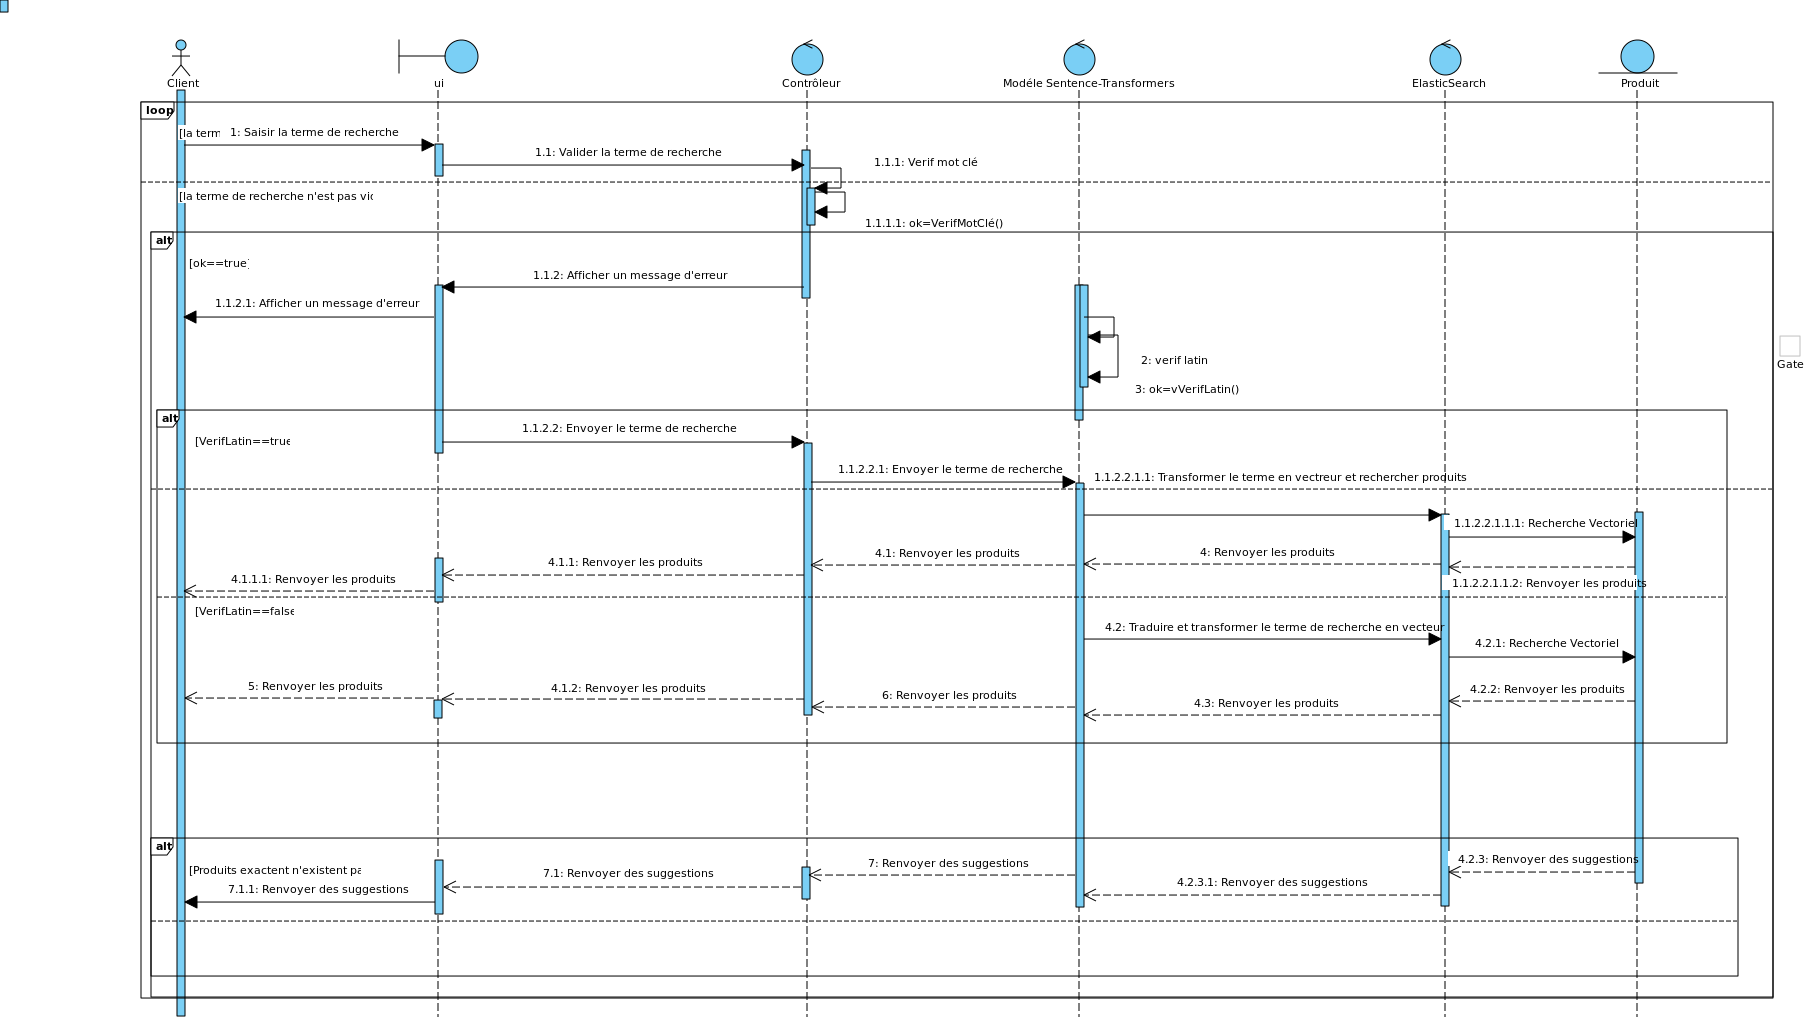
\includegraphics[width=1\textwidth]{logos/seqsprint2.png}
	\caption{Diagramme de séquence des cas d’utilisations « Rechercher produits en Arabe Traditionnel » et << Rechercher produits en Arabe en dialecte Tunisien >>}
	\label{fig:diagseqsprint2}
\end{figure}

\section{Réalisation}
\noindent
Cette partie est consacrée à la présentation des étapes nécessaires pour réaliser le travail nécessaire pour satisfaire notres cas d'utilisations, qui consiste à permettre le client ou le visiteur à rechercher notres produits en Arabe traditionnel et Arabe en dialecte tunisien tout en améliorant l'expérience de recherche en utilisant la traduction et la recherche vectorielle via Elasticsearch.

\newpage
\subsection{Les premières approches}
\noindent
Puisque notre modèle actuel n'est formé que sur les langues latines, nous avons eu l'idée de l'entraîner à la fois sur l'arabe tunisien et l'arabe traditionnel, mais un certain nombre de limitations nous empêchaient de le faire:

\begin{enumerate}
	\item Absence totale de jeux de données sur la langue arabe en dialecte Tunisien.
	\item Absence totale de jeux de données sur la langue Arabe Traditionnel.
	\item Le processus de l'entraînement nécessite une machine beaucoup plus puissante et une période de temps très longue afin de traiter correctement les 2 langues que nous avons citées.
\end{enumerate}

\noindent
Nous avons également testé avec le « Fine-Tuning » pour entraîner notre modéle, nous définissons ce processus comme suit: \\
\textit{Le << Fine-Tuning >> consiste à prendre un modèle d'apprentissage automatique pré-entraîné et à le former davantage sur un ensemble de données plus petit et ciblé. L'objectif du réglage fin est de conserver les capacités d'origine d'un modèle pré-entraîné tout en l'adaptant à des cas d'utilisation plus spécialisés.} \\ \citetitle{techtarget:finetuning} (\cite{techtarget:finetuning})

\noindent
Mais ce processus nécessitait un ensemble de données beaucoup plus volumineux que celui que nous avions préparé et prenait trop de temps, nous avons donc décidé d'adopter l'approche mentionnée ci-dessous.

\newpage
\subsection{Création de notre propre classe traducteur}
\noindent
Avec les limitations de l'approche << Fine-Tuning >> que nous avons mentionnée précédemment, nous avons décidé de créer notre propre traducteur qui va:
\begin{enumerate}
	\item Vérifier si le terme de recherche est en Arabe traditionnel, et le traduire en Français à partir de l'API Google Traduction.
	\item Vérifier si le terme de recherche est en Arabe en dialecte Tunisien à partir de notre propre dictionnaire des mots Tunisiens et leur equivalent en Français, si il n'y a pas d'équivalent exacte, il essaie de trouver l'équivalent en calculant un pourcentage, et s'il n'y a pas d'équivalent même après avoir calculé le pourcentage, le mot reste tel quel en supposant qu'il soit en Français
\end{enumerate}

\subsubsection{La création du dictionnaire}
\noindent
D'abord, nous commençons par préparer notre classe, que nous avons nommée << TunisianTranslator >> et initialiser un attribut privé, qui est notre dictionnaire. La figure ~\ref{fig:dictionary} montre le code nécessaire pour cette étape.

\begin{figure}[H]
	\centering
	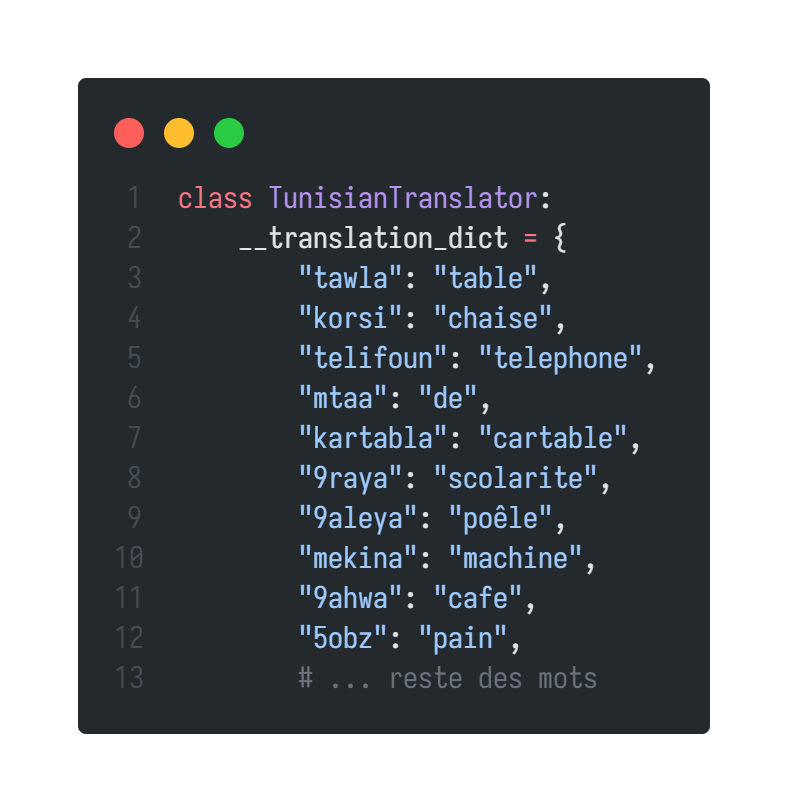
\includegraphics[width=0.6\textwidth]{logos/dictionary.png}
	\caption{Code d'initialisation de classe et du dictionnaire}
	\label{fig:dictionary}
\end{figure}

\noindent
Ensuite, nous continuons en définissant notre première méthode dans la classe qui est une méthode privée nommée \texttt{\_\_is\_latin}. Cette méthode est conçue pour vérifier si une chaîne donnée s contient uniquement des caractères des blocs Unicode Basic Latin et Latin-1 Supplement, elle renvoie True si tous les caractères de la chaîne << s >> se trouvent dans la plage Unicode U+0000 à U+00FF, ce qui correspond aux blocs Basic Latin et Latin-1 Supplement. Si un caractère se situe en dehors de cette plage, la méthode renvoie False.

\subsubsection{Analyse des expressions régulières}
\noindent
L'expression régulière utilisée dans notre méthode est :
\Large\[ [^{\backslash u0000-\backslash u00FF}] \]
\begin{itemize}
	\item \texttt{[...]}: Spécifie une classe de caractères, correspondant à n'importe quel caractère unique inclus entre parenthèses.
	\item \texttt{\^{}}: Entre parenthèses de classe de caractères, cela annule la classe, donc elle correspond à n'importe quel caractère \emph{non} répertorié entre parenthèses.
	\item \texttt{\textbackslash u0000-\textbackslash u00FF}: Définit une plage de caractères Unicode de \( U+0000 \) à \( U+00FF \), qui comprend à la fois les blocs Basic Latin et Latin-1 Supplement.
\end{itemize}

\newpage
\noindent
Le \texttt{Latin-1 Supplement} est défini comme suit: \\
\textit{Le bloc Latin-1 Supplement fait partie de la norme Unicode, couvrant la plage de \( U+0080 \) jusqu'à \( U+00FF \). Il complète le bloc Basic Latin (ASCII), qui couvre de \( U+0000 \) jusqu'à \( U+007F \). Ce bloc comprend des caractères supplémentaires utilisés dans diverses langues occidentales, comprenant des lettres accentuées, des signes de ponctuation, des symboles monétaires et d'autres symboles typographiques, représentant la moitié supérieure du codage de caractères ISO/IEC 8859-1.} \\
\citetitle{symbl:latin1supp} (\cite{symbl:latin1supp})


\subsubsection{Logique de méthode}
\noindent
La méthode \texttt{re.search(r"[\textbackslash u0000-\textbackslash u00FF]", s)} recherche dans la chaîne \( s \), recherchant tout caractère en dehors de plage \( U+0000 \) jusqu'à \( U+00FF \):
\begin{itemize}
	\item Si un tel caractère est trouvé, \texttt{re.search} renvoie un objet de correspondance, qui est évalué à \texttt{True}.
	\item Si aucun caractère de ce type n'est trouvé (c'est-à-dire que tous les caractères sont dans la plage spécifiée), il renvoie \texttt{None}, qui est évalué à \texttt{False}.
\end{itemize}
L'utilisation de l'opérateur \texttt{not} inverse le résultat de \texttt{re.search}. Ainsi, la méthode renvoie \texttt{False} si des caractères se trouvent en dehors de la plage Unicode spécifiée, et \texttt{True} si tous les caractères s'y trouvent.

\noindent
La figure ~\ref{fig:islatin} illustre le code nécessaire pour cette méthode.

\begin{figure}[H]
	\centering
	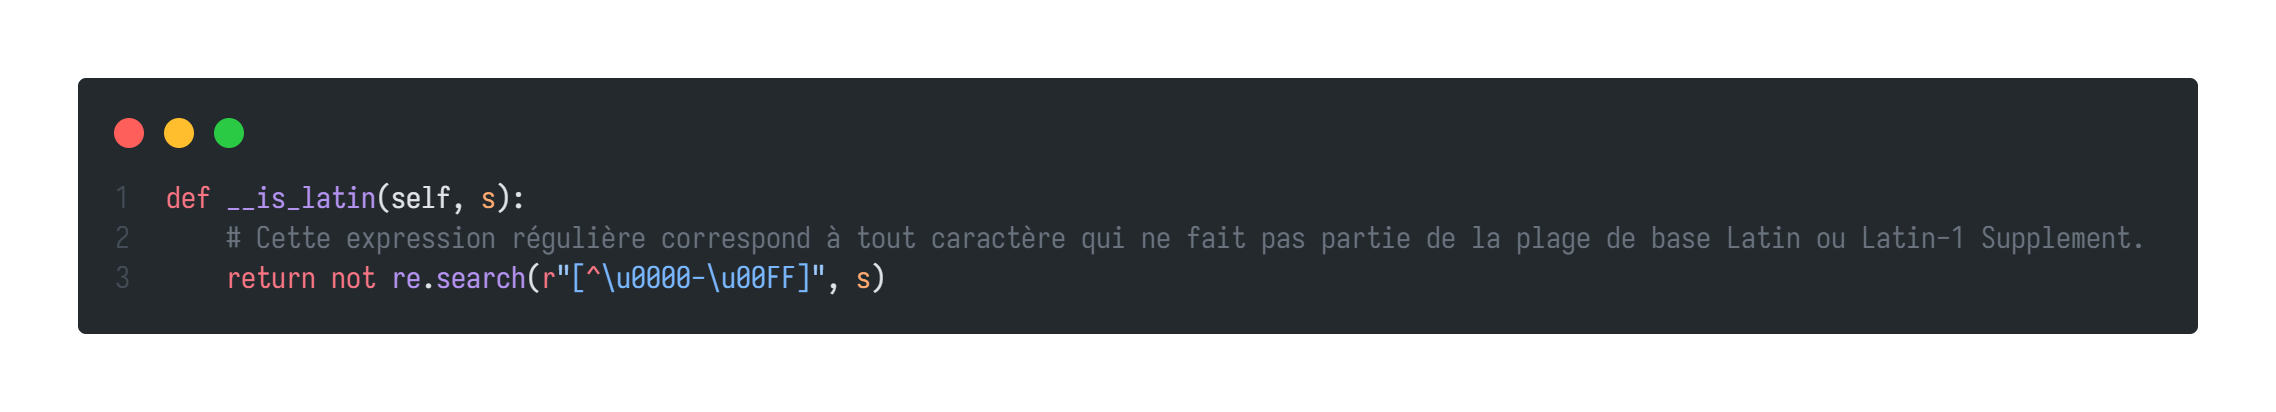
\includegraphics[width=1\textwidth]{logos/islatin.png}
	\caption{Code de méthode \_\_is\_latin}
	\label{fig:islatin}
\end{figure}

\noindent
Cette méthode étant terminée, nous passons maintenant à notre deuxième méthode, qui est une méthode privée appelée \texttt{\_\_find\_best\_match} pour vérifier le mot correspondant le plus proche dans notre dictionnaire Tunisien. \\
Pour avoir cette fonctionnalité, on va utiliser la bibliothéque \texttt{difflib} du langage de programmation Python, qui fournit des aides pour calculer les différences entre les séquences, y compris des outils pour trouver des séquences correspondant étroitement à une séquence d'entrée donnée.

\subsubsection{Répartition des fonctionnalités}
\noindent
Pour trouver cette mot correspondant, on va utiliser la méthode \\
\texttt{get\_closest\_matches} qui prends 4 paramétres:
\begin{enumerate}
	\item \texttt{tunisian\_text:} La chaîne de caractères pour laquelle des correspondances proches sont recherchées.
	\item \texttt{self.\_\_translation\_dict.keys():} La séquence à laquelle le tunisian\_text est comparé. Ici, ce sont les clés du notre dictionnaire Tunisien \_\_translation\_dict.
	\item \texttt{n=1:} Ce paramètre spécifie le nombre de correspondances proches à renvoyer. Le réglage n=1 signifie que la fonction renverra au plus une correspondance la plus proche.
	\item \texttt{cutoff=0.7:} C'est le seuil de similarité. Les correspondances avec un score de similarité inférieur à 0,7 (où 1,0 correspond à une correspondance exacte et 0 à une absence de similarité) ne sont pas incluses. Une valeur de 0,7 implique que la fonction prendra en compte les correspondances qui sont similaires à au moins 70 à tunisian\_text.
\end{enumerate}

\subsubsection{Renvoie du rèsultat}
\noindent
La fonction sauveguarde les résultats de \texttt{get\_close\_matches} dans la variable \texttt{matches}, elle vérifie ensuite si des correspondances ont été trouvées. Si \texttt{matches} contient des éléments, \texttt{matches[0]} (la meilleure correspondance due à n=1) est renvoyé. Si \texttt{matches} est vide, ce qui indique qu'aucune correspondance suffisamment proche n'a été trouvée, la méthode renvoie None.\\ La figure ~\ref{fig:findbestmatch} illustre le code nècessaire pour cette mèhode.

\begin{figure}[H]
	\centering
	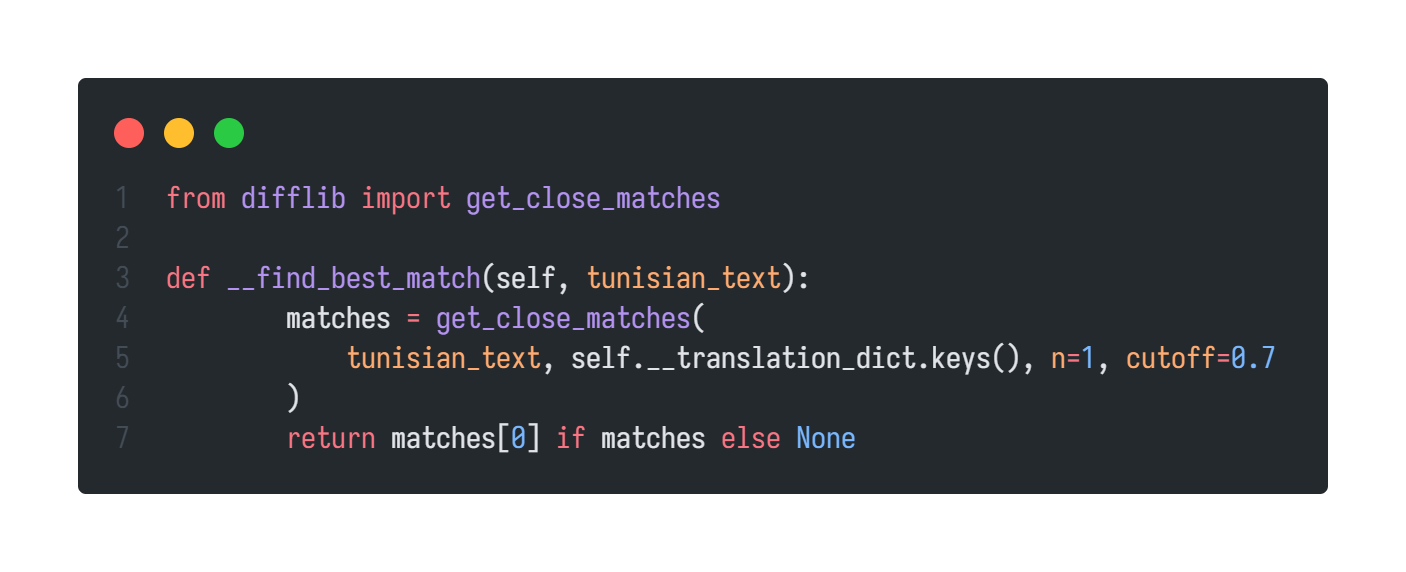
\includegraphics[width=1\textwidth]{logos/findbestmatch.png}
	\caption{Code de méthode \_\_find\_best\_matches}
	\label{fig:findbestmatch}
\end{figure}

\newpage
\noindent
Une fois les 2 méthodes précédentes sont terminées, nous pouvons maintenant passer à notre méthode la plus importante, qui utilisera ces méthodes pour gérer la logique de traduction et renverra le terme de recherche traduit. La méthode est appelé \texttt{translate}, et sa visibilité est publique.

\subsubsection{Aperçu de la méthode}
\noindent
\textit{But:} Traduire du texte du tunisien ou ou du texte en Arabe traditionnel (non latin) vers le Français,, en utilisant à la fois des services de traduction automatisée et un dictionnaire de traduction prédéfini. \\
\textit{Input:} \texttt{text:} Une chaîne de caractères contenant le texte à traduire. \\
\textit{Output:} Le texte traduit en Français, ou un message d'erreur si la traduction échoue.

\newpage
\subsubsection{Répartition détaillée}
\begin{enumerate}
	\item Initialisation des variables:
	      \begin{itemize}
		      \item \texttt{mots = [] :} Initialise une liste vide qui contiendra plus tard des mots individuels du texte saisi.
	      \end{itemize}
	\item Vérifiez les caractères non latins:
	      \begin{itemize}
		      \item On utilise la méthode \texttt{\_\_is\_latin} pour vérifier si le texte est en latin ou non. Si cette méthode renvoie \texttt{False}, nous utilisons Google Traduction pour traduire ce texte en Français, sinon, nous vérifions si le texte est en Tunisien en vérifiant si il y'a une correspondance dans notre dictionnaire.
	      \end{itemize}
	\item Utilisation de Google Traduction
	      \begin{itemize}
		      \item Création de l'instance de l'objet \texttt{Translator} importé de la bibliothéque \texttt{googletrans}.
		      \item La méthode essaie de traduire le texte en Français (dest="fr"). En cas de succès, le texte du résultat traduit remplace le texte original.
	      \end{itemize}
	\item Traduction en utilisation de notre dictionnaire
	      \begin{itemize}
		      \item Nous initialisons une liste vide pour stocker les mots traduits (translated\_words = []).
		      \item Ensuite, nous performons une itération sur les mots de terme de recherche.
		      \item Recherche de la meilleure correspondance : pour chaque mot, il appelle self.\_\_find\_best\_match(word) pour trouver la clé correspondante la plus proche dans le dictionnaire de traduction \_\_translation\_dict.
		      \item Si une correspondance est trouvée (la clé n'est pas None), la méthode ajoute la valeur correspondante de \_\_translation\_dict à translated\_words.
		      \item Si aucune correspondance n'est trouvée, le mot original est ajouté à translated\_words car elle suppose que le mot n'a pas besoin de traduction ou qu'aucune traduction appropriée n'existe dans le dictionnaire, supposons qu'elle est en Français.
	      \end{itemize}
		\item Construction de la phrase traduite finale en joignant la liste translated\_words en une seule chaîne avec des mots séparés par des espaces (" ".join(translated\_words)) et renvoie cette chaîne comme phrase traduite finale.
\end{enumerate}

\newpage
\noindent
La figure ~\ref{fig:translate} illustre le code nècessaire pour créer cette méthode.

\begin{figure}[H]
	\centering
	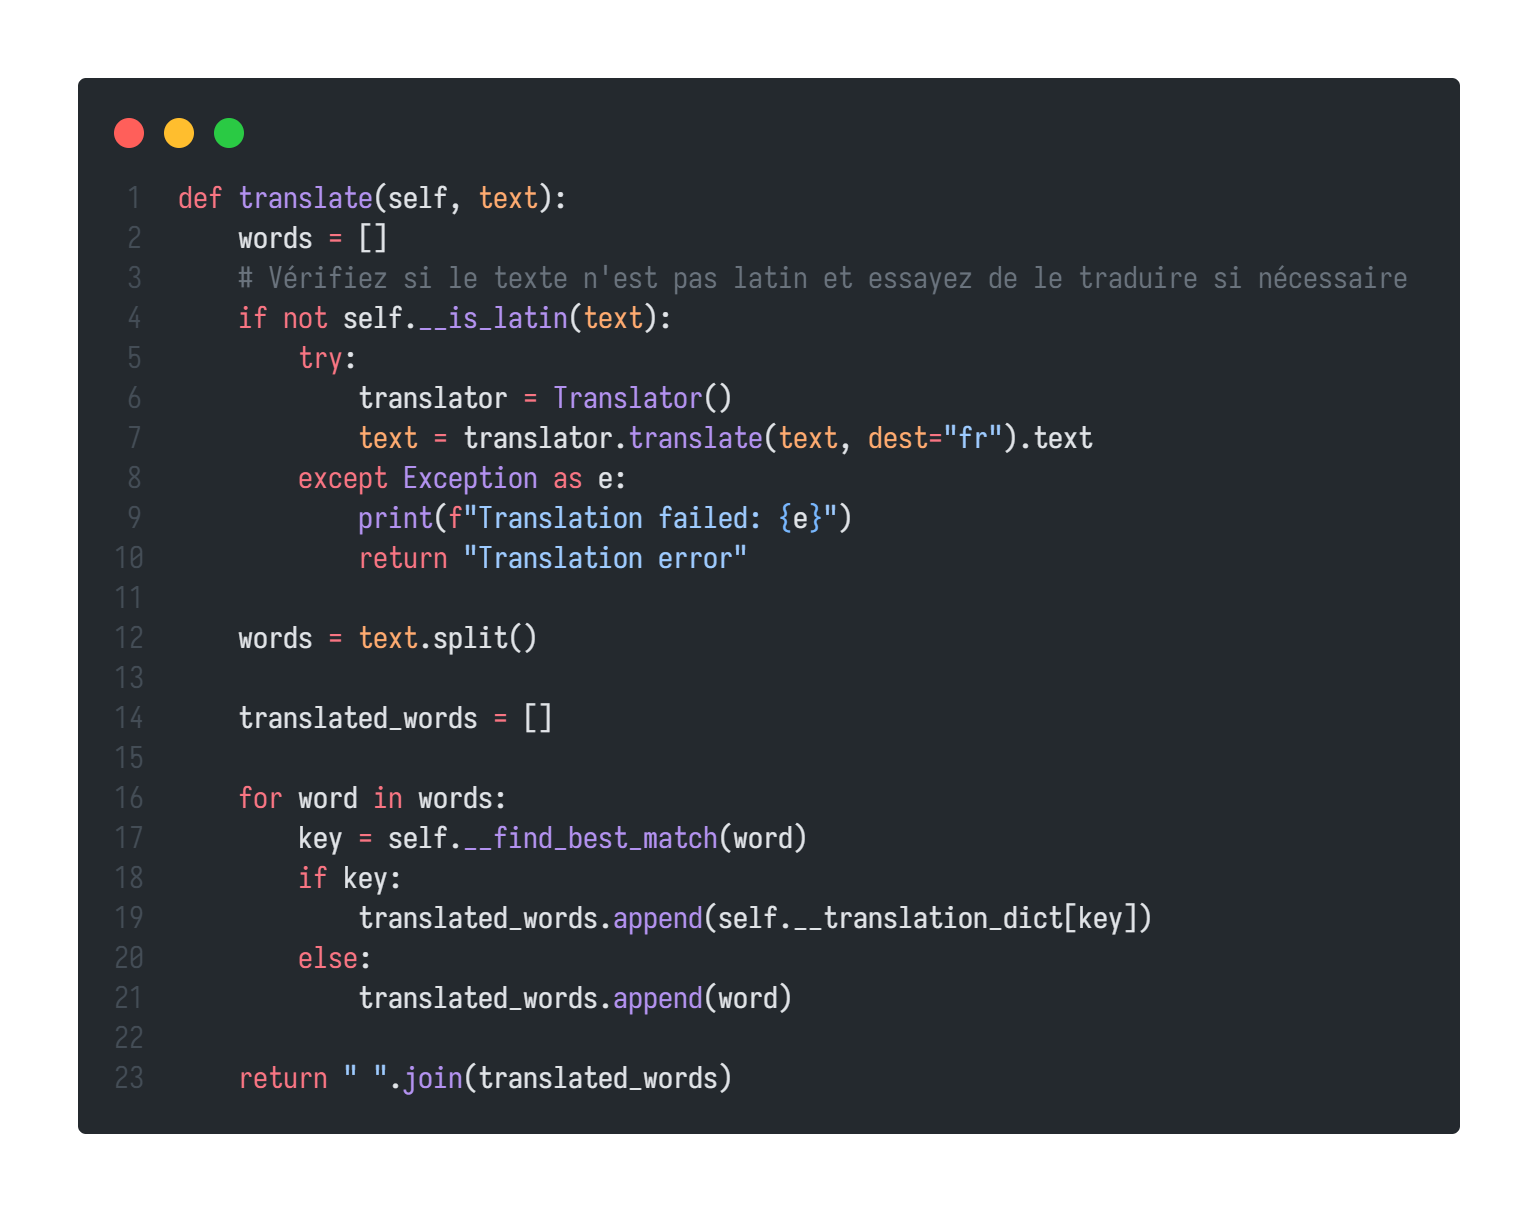
\includegraphics[width=1\textwidth]{logos/translate.png}
	\caption{Code de méthode translate}
	\label{fig:translate}
\end{figure}

\noindent
Enfin, nous doivent exposer une endpoint Flask \texttt{"/encode"} comme une endpoint de microservice publique pour regrouper toutes le fonctionnalités qui sont les suivants:
\begin{enumerate}
	\item Extraire le terme de recherche de la requête.
	\item Essayez de le traduire en Français si nécessaire.
	\item Utiliser la méthode encode\_sentence\_and\_normalise de notre modéle Sentence-Transformers pour faire l'encodage du terme de recherche en vecteur.
	\item Renvoyer ce vecteur au contrôleur ASP .NET Core sous forme JSON.
\end{enumerate}

La figure ~\ref{fig:encodeendpoint} illustre le code complèt du endpoint \texttt{"/encode"}.

\begin{figure}[H]
	\centering
	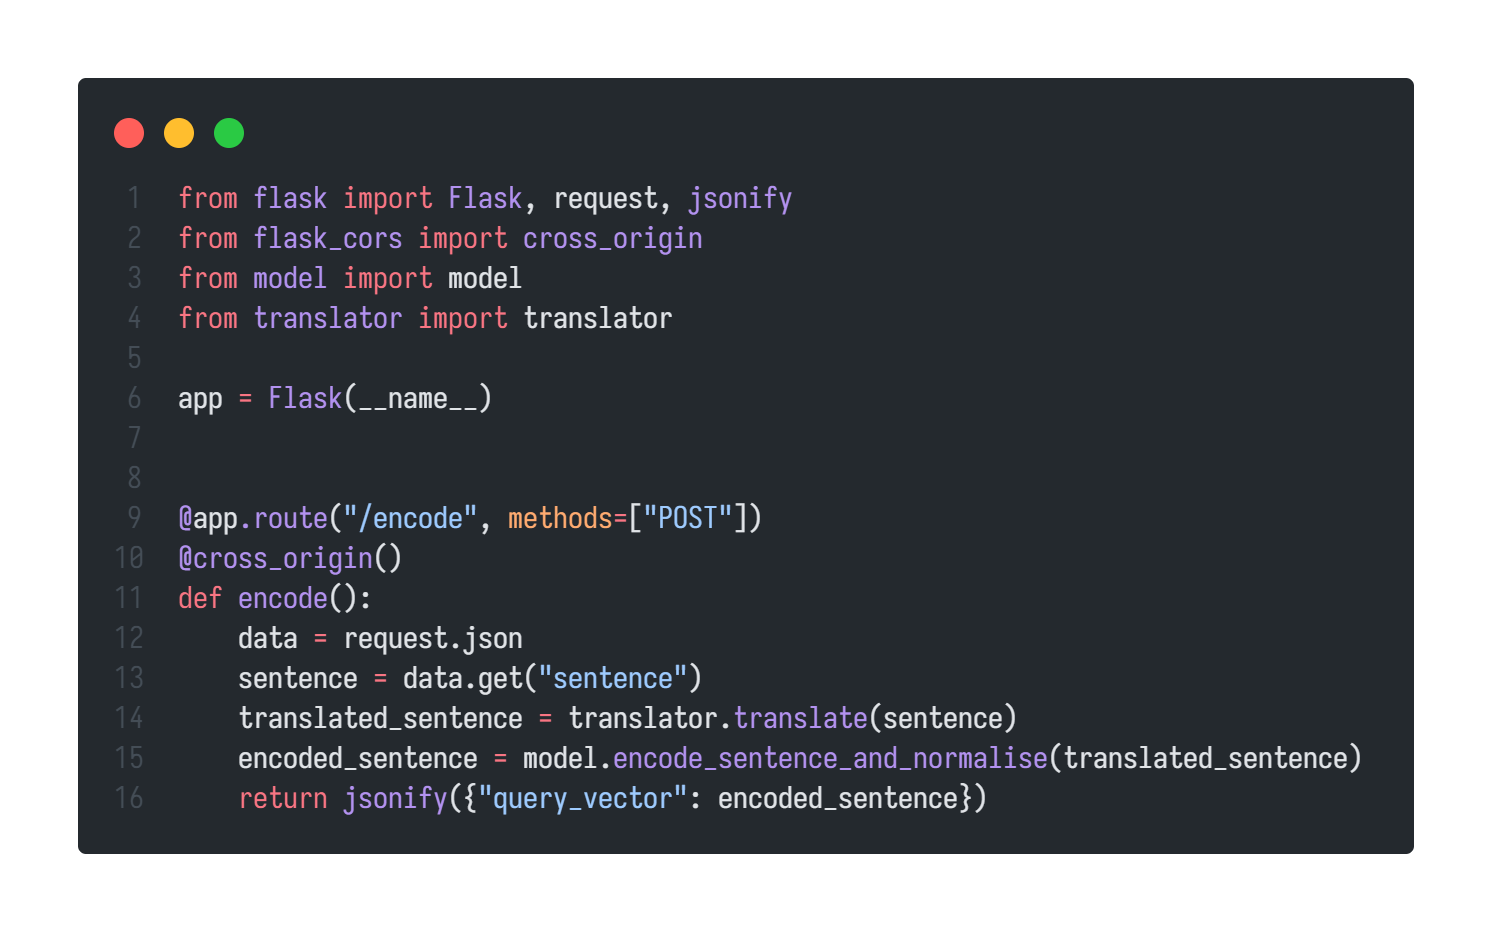
\includegraphics[width=1\textwidth]{logos/encodeendpoint.png}
	\caption{Code de endpoint "/encode"}
	\label{fig:encodeendpoint}
\end{figure}

\newpage
\noindent
\section{Processus complèt de recherche vectorielle avec la traduction}
\noindent
La figure ~\ref{fig:fullprocesswithtranslation} illustre le processus complèt de recherche vectorielle avec la traduction.

\begin{figure}[H]
	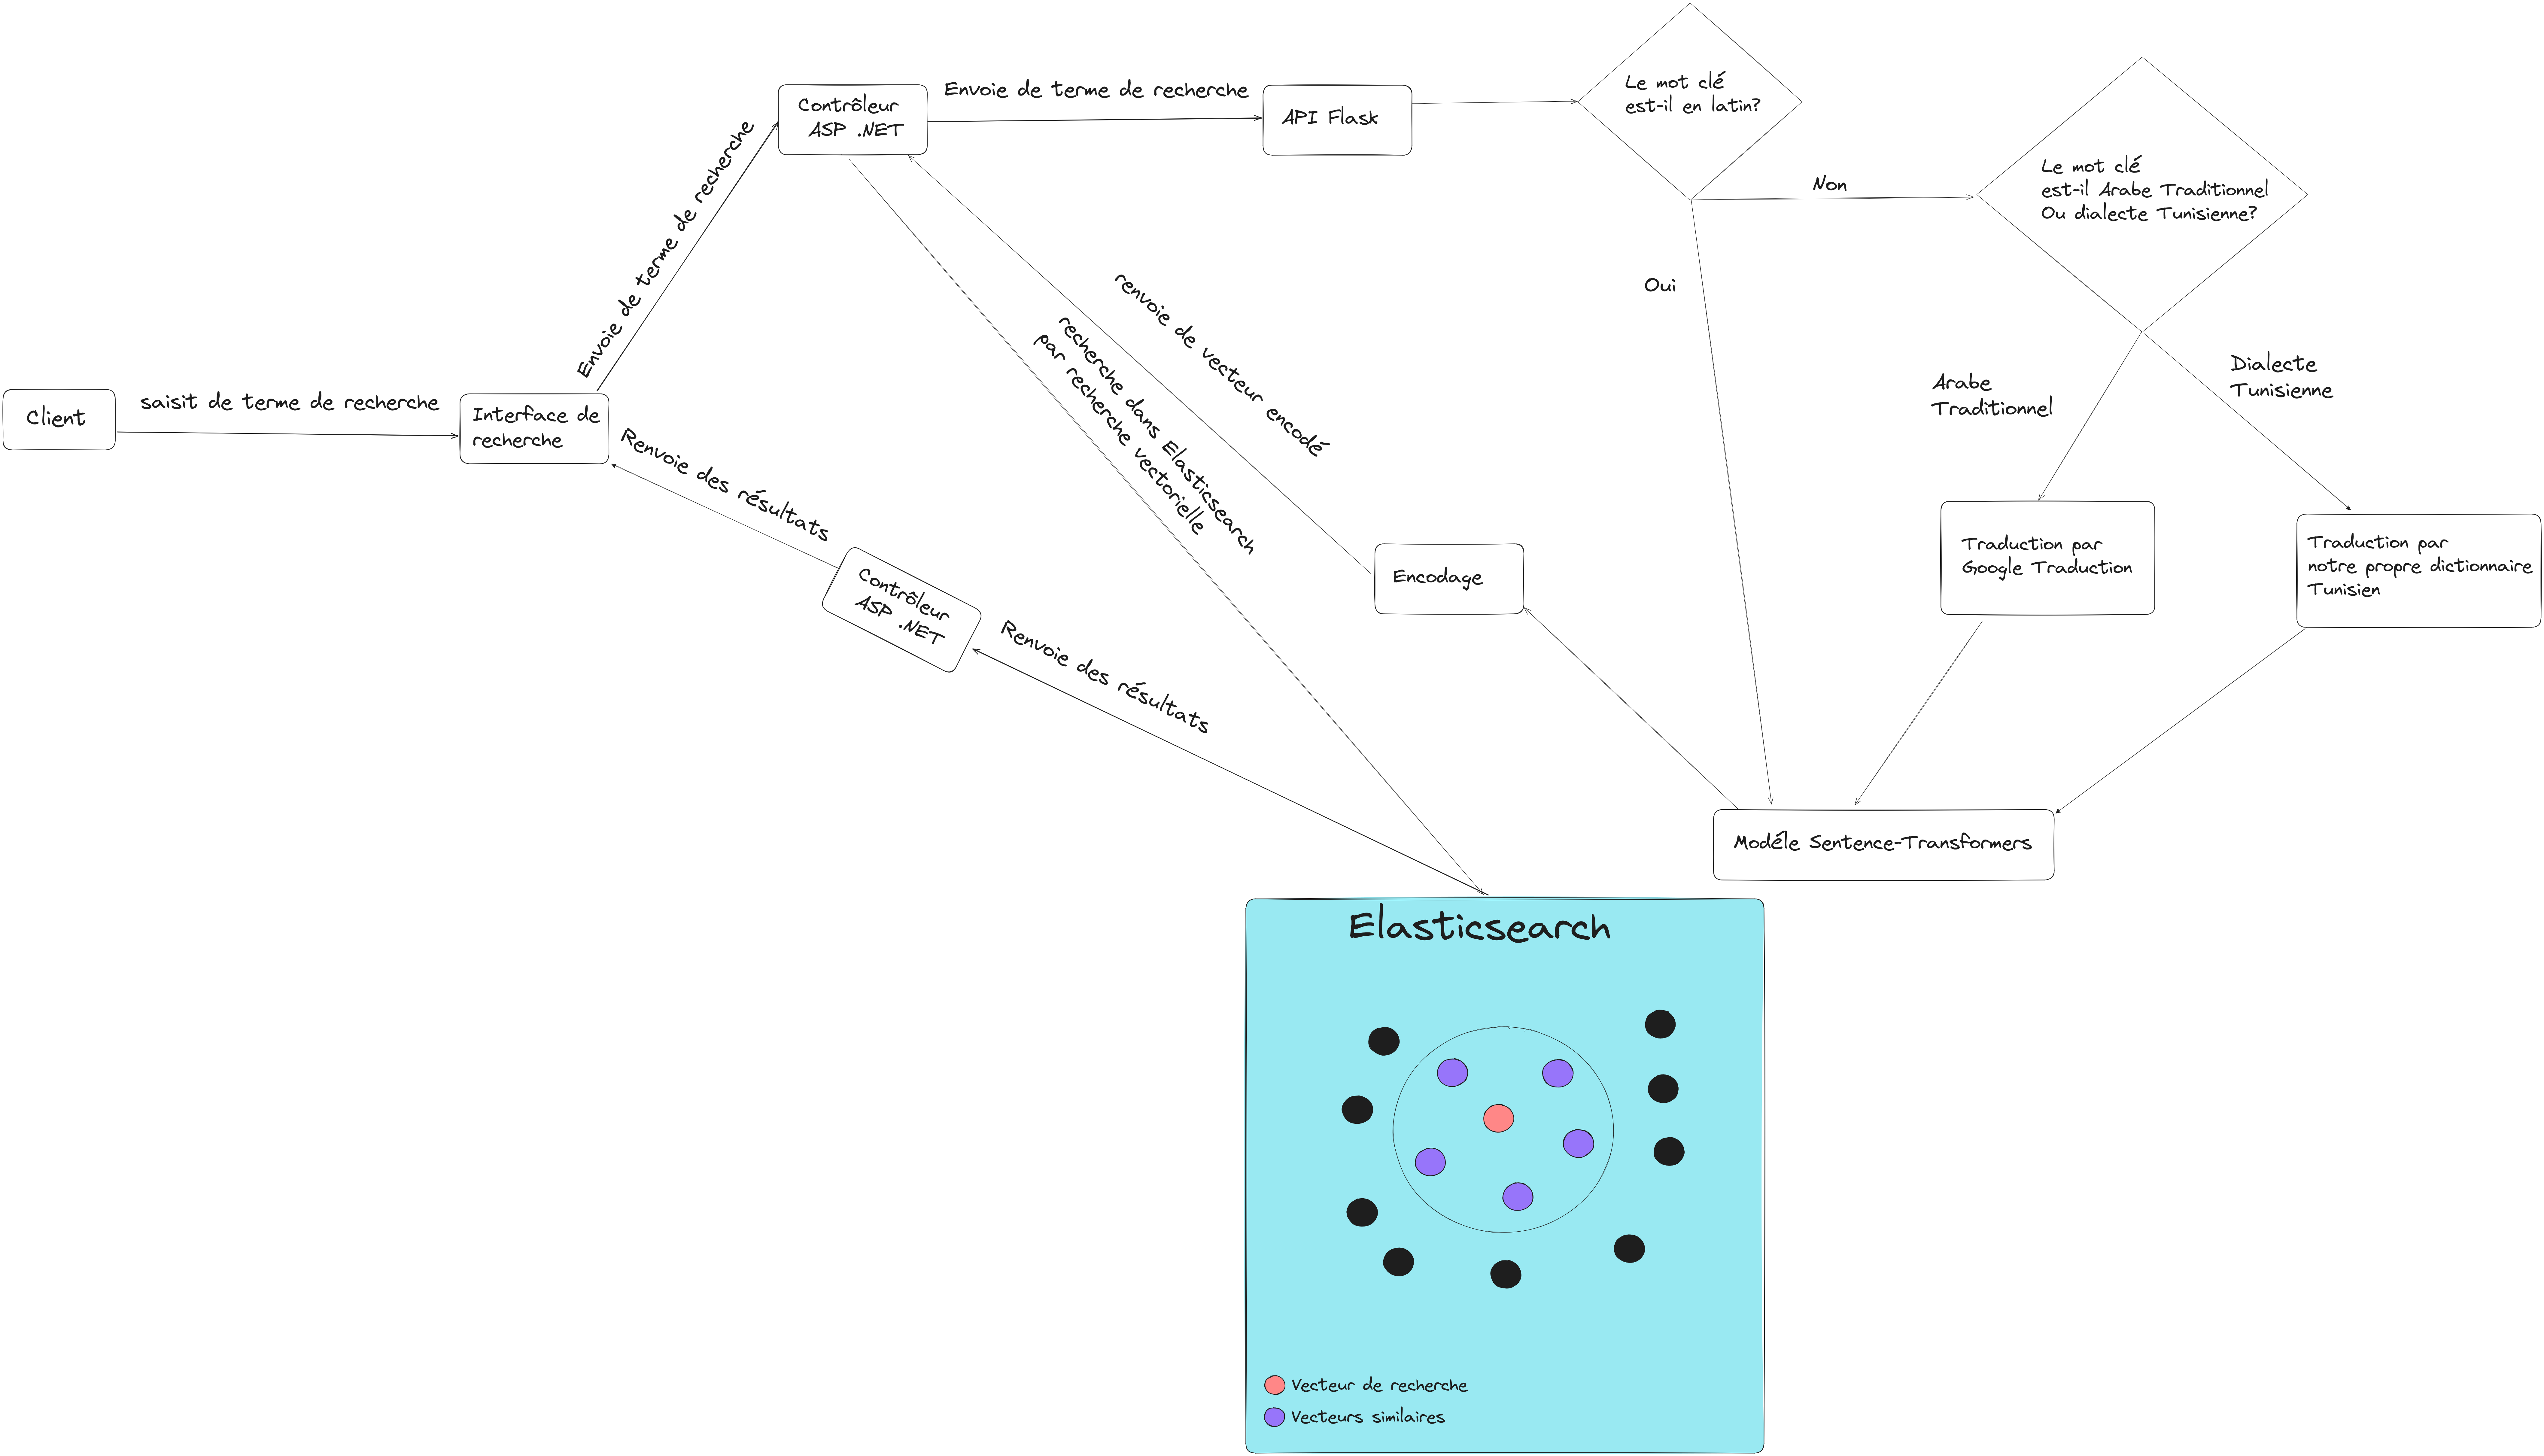
\includegraphics[width=1\textwidth]{logos/fullprocesswithtranslation.png}
	\caption{Processus complèt de recherche vectorielle avec la traduction}
	\label{fig:fullprocesswithtranslation}
\end{figure}

\subsection{Rèpartition dètaillèe de processus de recherche vectorielle complèt}
\begin{enumerate}
	\item \texttt{Intèraction du client:} Le client saisit son terme de recherche à travers l'interface de recherche.
	\item \texttt{Contrôleur ASP.NET :} Contrôleur ASP.NET : le terme de recherche est envoyé du client à un contrôleur backend implémenté dans ASP.NET, qui transmet ensuite le terme de recherche à une API Flask.
	\item \texttt{Analyse des mots clés:} l'API Flask détermine si le terme de recherche est en latin. Si tel est le cas, le processus passe directement à l'encodage du terme en utilisant notre modéle Sentence-Transformers pour qu'il soit adapté à la recherche vectorielle dans Elasticsearch. Si le terme n'est pas en latin, il vérifie s'il est en arabe traditionnel ou en dialecte tunisien, sinon, il suppose qu'il est en Français.
	\item \texttt{Traduction selon la langue détectée:} Les termes arabes traditionnels sont traduits à l'aide des services de traduction Google. Les termes du dialecte tunisien sont traduits à l'aide de notre dictionnaire tunisien.
	\item \texttt{Encodage}: Les termes traduits sont éventuellement codés à l'aide de notre modéle Sentence-Transformers.
	\item \texttt{Recherche vectorielle dans Elasticsearch:} Les vecteurs codés sont utilisés pour interroger Elasticsearch, qui recherche des vecteurs (documents) similaires stockés dans son index, qui sont notre produits dans notre cas.
	\item \texttt{Récupération des résultats:} Les résultats de la recherche sont récupérés et renvoyés via le contrôleur ASP.NET au client, complétant ainsi le processus de recherche.
\end{enumerate}


\subsection{Interface de recherche et affichage des suggestions}
\noindent
Cette section est consacrée pour la réalisation de l'interface de recherche pour le client et le visiteur ainsi que l'affichage des suggestions des produits similaires a son terme de recherche. \\

\noindent
La figure ~\ref{fig:interfacerecherche} illustre l'interface de recherche, dans ce cas un visiteur a cherché pour parfum en Arabe traditionnel, et les résultats sont renvoyés, ainsi que des suggestions au bas de la page qui sont dans la figure ~\ref{fig:suggestions}.


\begin{figure}[H]
	\centering
	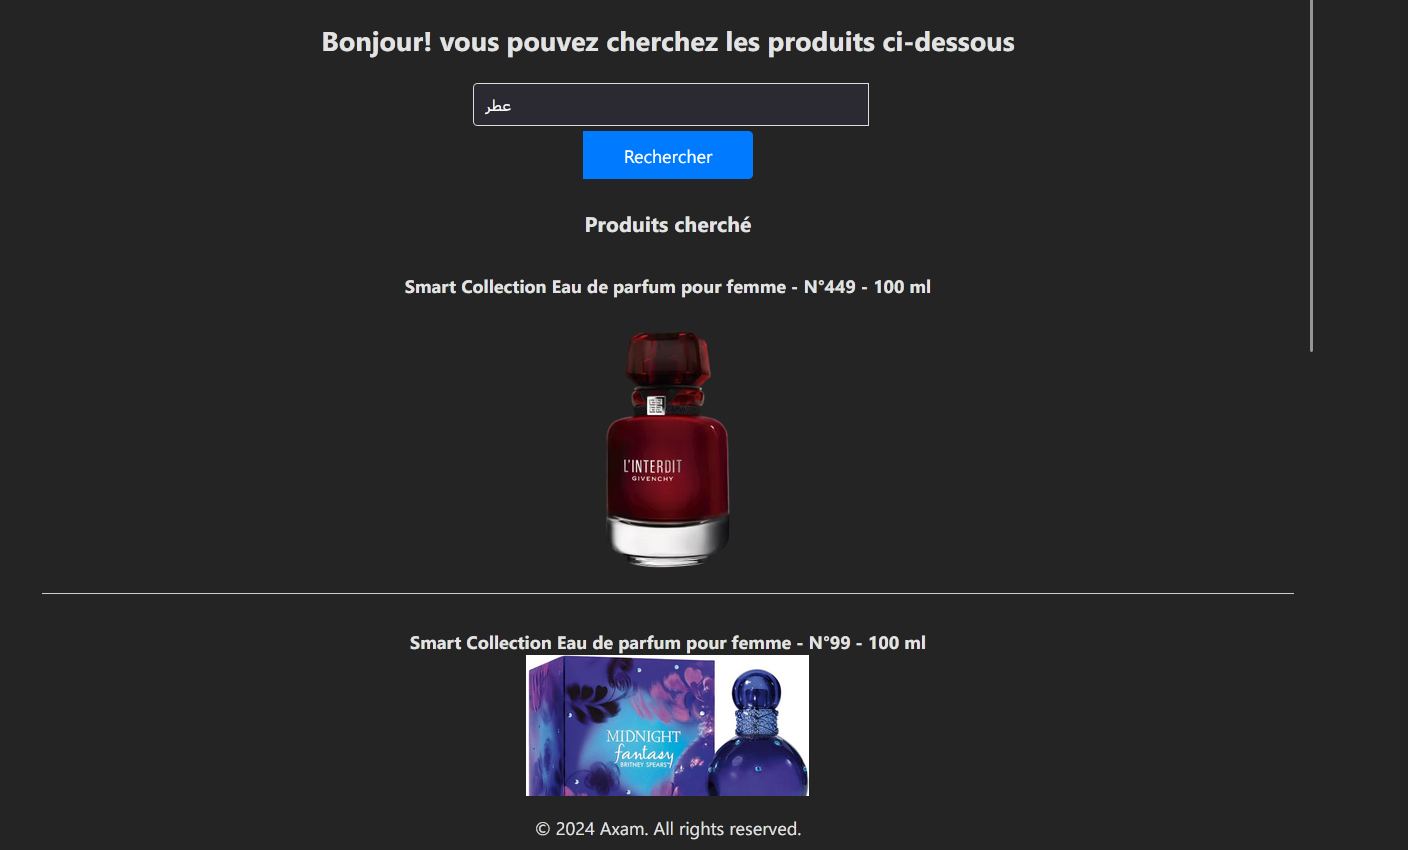
\includegraphics[width=1\textwidth]{logos/interfacerecherche.png}
	\caption{Interface de recherche de client et visiteur}
	\label{fig:interfacerecherche}
\end{figure}

\begin{figure}[H]
	\centering
	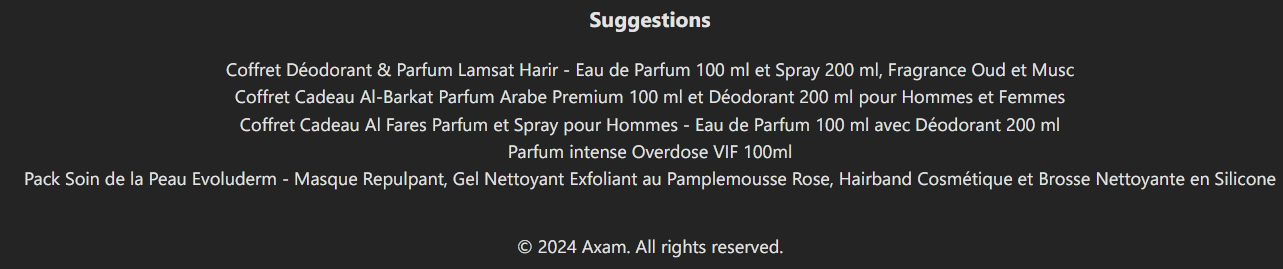
\includegraphics[width=1\textwidth]{logos/suggestions.png}
	\caption{Affichage des suggestions des noms des produits similaires}
	\label{fig:suggestions}
\end{figure}


\section{Conclusion}
\noindent
Dans ce chapitre, nous avons couvert toutes les étapes nécéssaires pour permettre le client à rechercher notres produits en Arabe traditionnel et en dialecte Tunisien a travers le processus de traduction et traitement du mot clé qu'il cherche en utilisant les divers techniques, fonctions et bibliothéque mentionné tout au long de notre chapitre.
